\section{Análisis de performance}
\subsection{Aclaraciones}
Para generar los siguientes análisis de performance, se creó un programa en \textit{Python} para generar una serie de problemas a computar, con y sin solución, desde $10$ hasta $n$ elementos. Se pueden describir los problemas como elementos de una matriz $Problema \ problemas[n][r]$ donde $Problema$ es una tupla del tipo $(T, values)$, $n$ es la cantidad máxima de elementos a evaluar y $r$ es la cantidad de repeticiones para cada problema de tamaño $n$. Es decir, la cantidad de veces que se va a repetir un experimento de $n$ elementos con el objetivo de mejorar las mediciones obtenidas. Es necesario aclarar que para toda repetición de un problema dado un $n$, sus valores $T$ serán iguales. Esto es necesario para poder estimar confiablemente la equivalencia de un cómputo $\mathcal{O}(1)$ en segundos. Esto se realiza dividiendo el valor de $T$ contra la cantidad de recursiones que demandó cada problema. De esta manera, se obtiene una cota $\mathcal{O}(n*T)$ aproximada en los análisis de programación dinámica.

\vskip 8pt

Además, cada problema es generado aleatoriamente con un $T$ entre $(999, 99999999)$. La mitad de los problemas tienen garantizada una solución. La otra mitad, no. La disposición de los elementos de los valores de $values$ con solución son equiprobables. Es decir, tienen los elementos que forman parte de la solución pueden estar en cualquier lugar de la lista. Es por eso que en algunos gráficos se podrá observar que ciertos problemas de $n$ elementos hayan sido solucionados más rápidamente que otros problemas de $k$ elementos, con $n > k$. Estos casos intentan ser apaciguados mediante la elevada repetición de los problemas para cada cardinal y luego a través de la "poda" del $5\%–10\%$ de las soluciones más rápidas para cada tamaño de problema.

\vskip 8pt

Específicamente, los experimentos fueron computados para $n = 10 ... 34$ con $r = 40$. Es decir, cada $n$ fue calculado 40 veces con el mismo $T$ pero distintas listas de valores de $n$ elementos.

\subsection{Fuerza Bruta}
\begin{figure}[H]
	\centering
	\begin{minipage}{0.48\textwidth}
		\centering
		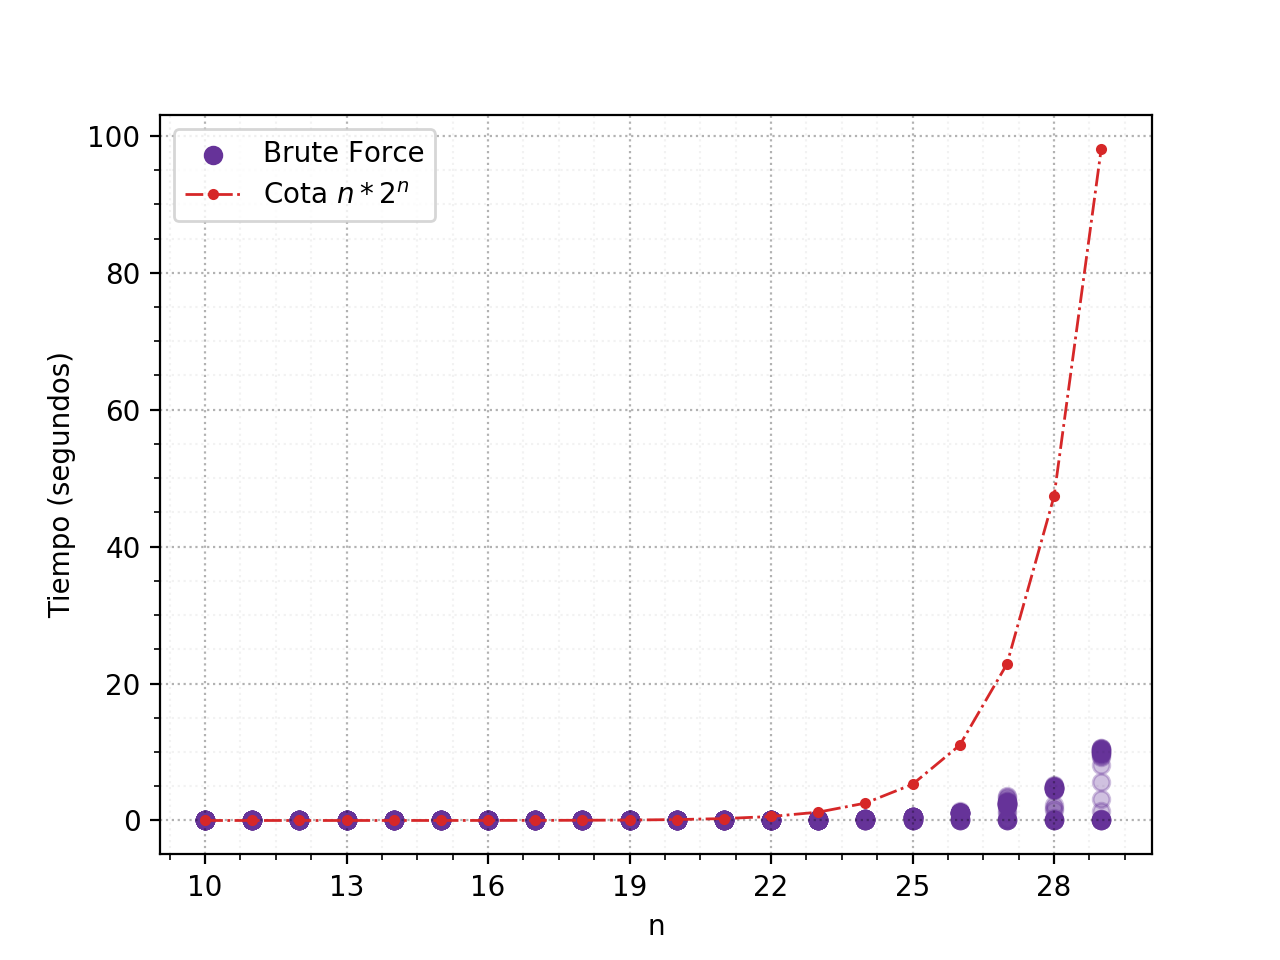
\includegraphics[width=1\textwidth]{bf-and-cota}
		\caption{\footnotesize Segundos consumidos (en escala lineal) en función de la cantidad de elementos de $values$.}
		\label{fig:plot-bf-and-cota}
	\end{minipage}%
	\hspace{0.03\textwidth}
	\begin{minipage}{0.48\textwidth}
		\centering
		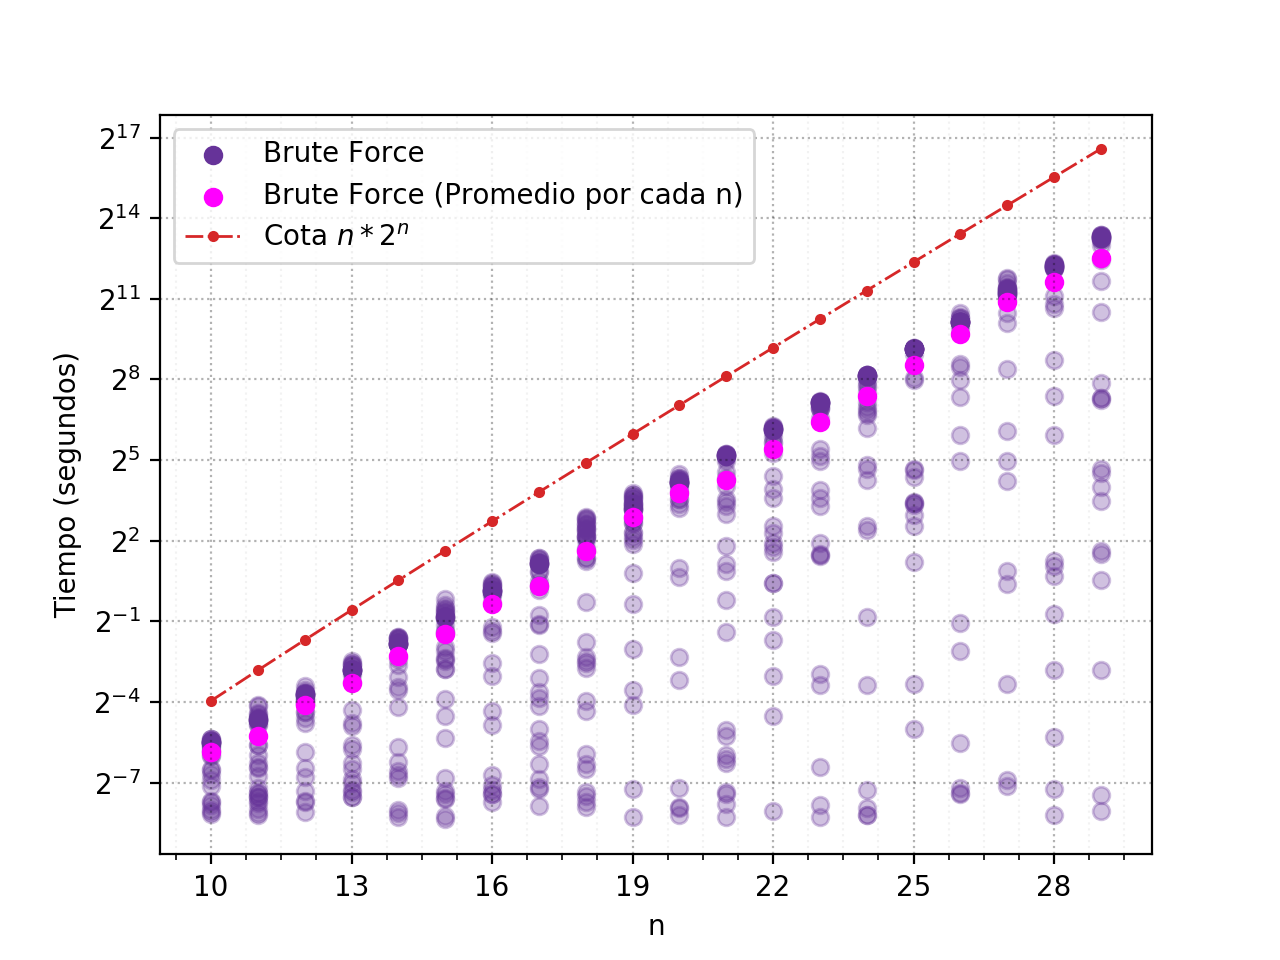
\includegraphics[width=1\textwidth]{bf-and-cota-log}
		\caption{\footnotesize Segundos consumidos (en escala logarítmica) en función de la cantidad de elementos de $values$.}
		\label{fig:plot-bf-and-cota-log}
	\end{minipage}%
\end{figure}

En estos gráficos se puede observar – en púrpura – todas las computaciones para cada problema de cardinal $n$. Mientras que, en rojo, se puede apreciar la cota teórica del algoritmo de fuerza bruta. Ambos experimentos apoyan empíricamente la hipótesis "\textit{El algoritmo de fuerza bruta tiene complejidad} $\mathcal{O}(n*2^n)$". Además, queda claro el comportamiento exponencial de la solución. Esta hipótesis puede ser reforzada con el siguiente experimento:

\begin{figure}[H]
	\centering
	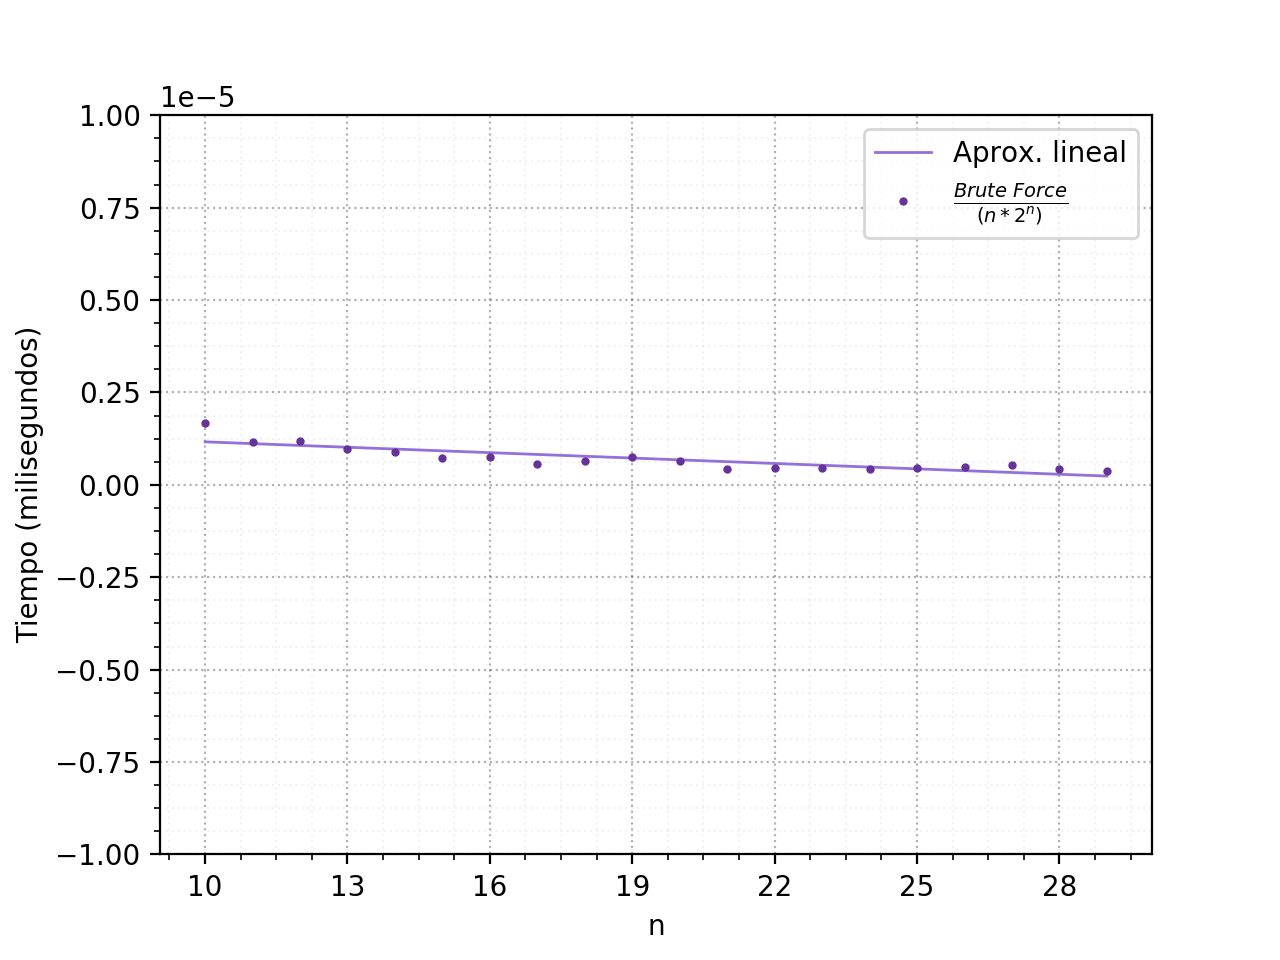
\includegraphics[width=0.5\textwidth]{bf-div-cota}
	\caption{\footnotesize Segundos consumidos en función de la cantidad de elementos de $values$ dividido $n*2^n$}
	\label{fig:plot-bf-div-cota}
\end{figure}

De esta manera, queda explicitada la tendencia de la complejidad del algoritmo con respecto a su complejidad: siempre será ampliamente menor.

\subsection{Back Tracking}
\begin{figure}[H]
	\centering
	\begin{minipage}{0.48\textwidth}
		\centering
		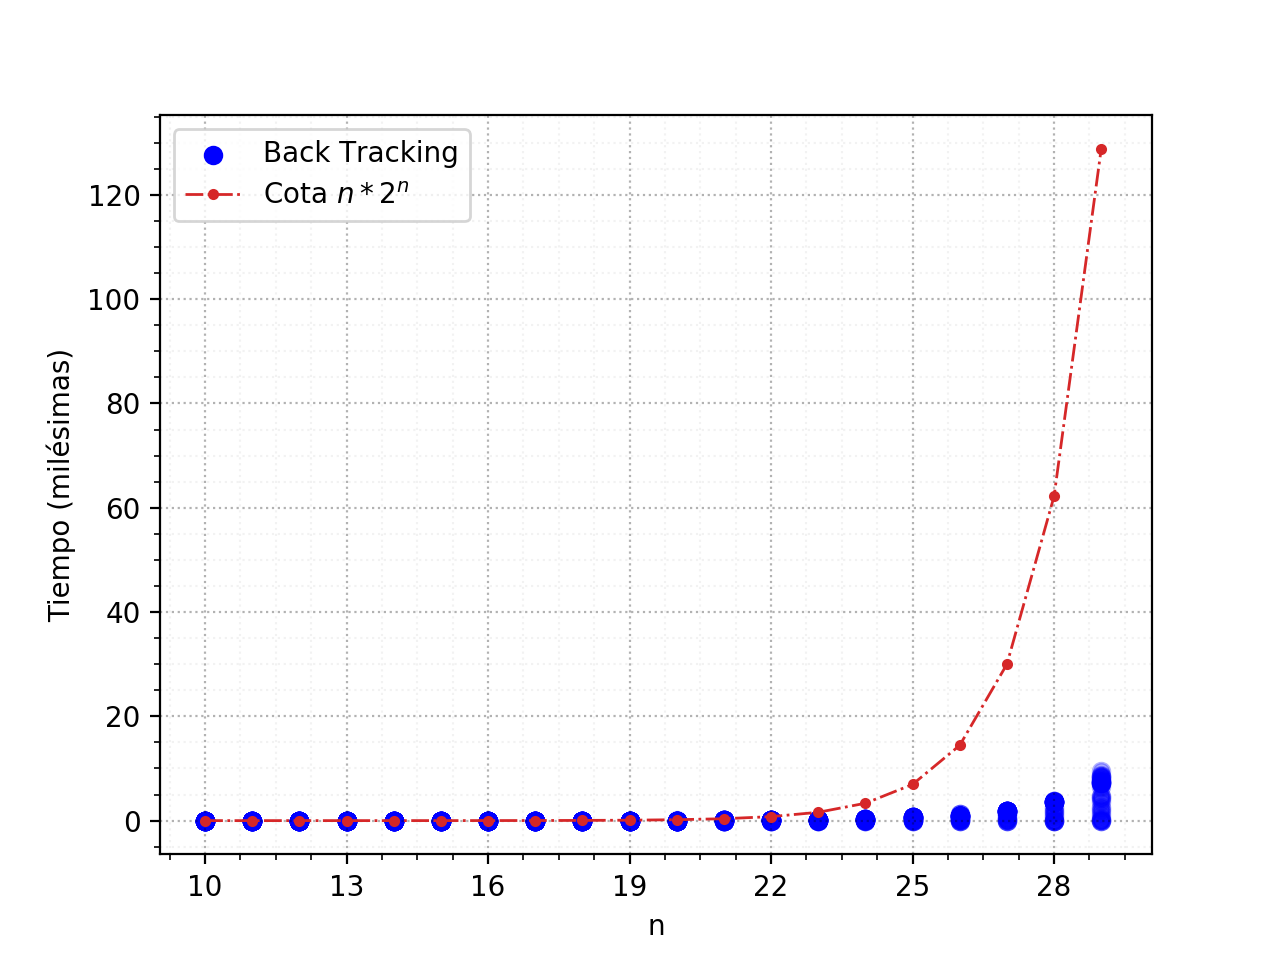
\includegraphics[width=1\textwidth]{bt-and-cota}
		\caption{\footnotesize Segundos consumidos (en escala lineal) en función de la cantidad de elementos de $values$.}
		\label{fig:plot-bt-and-cota}
	\end{minipage}%
	\hspace{0.03\textwidth}
	\begin{minipage}{0.48\textwidth}
		\centering
		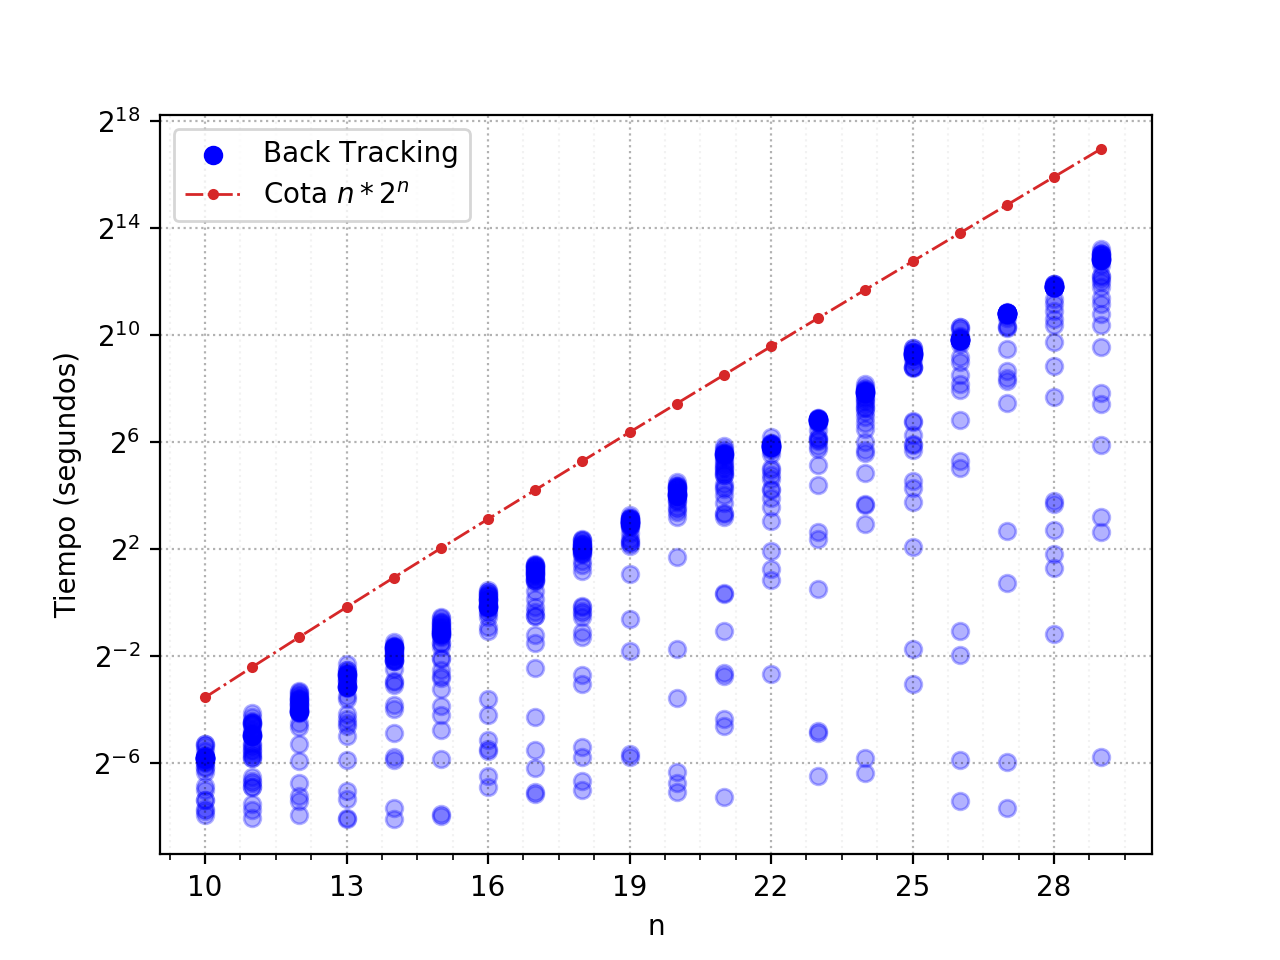
\includegraphics[width=1\textwidth]{bt-and-cota-log}
		\caption{\footnotesize Segundos consumidos (en escala logarítmica) en función de la cantidad de elementos de $values$.}
		\label{fig:plot-bt-and-cota-log}
	\end{minipage}%
\end{figure}

Al igual que en los gráficos de fuerza bruta, la tendencia es clara: la función $f(n)=n*2^n$ acota superiormente al algoritmo de back tracking para todo $n \in \{10, ..., 34\}$. A su vez, queda evidenciado su comportamiento exponencial.

\begin{figure}[H]
	\centering
	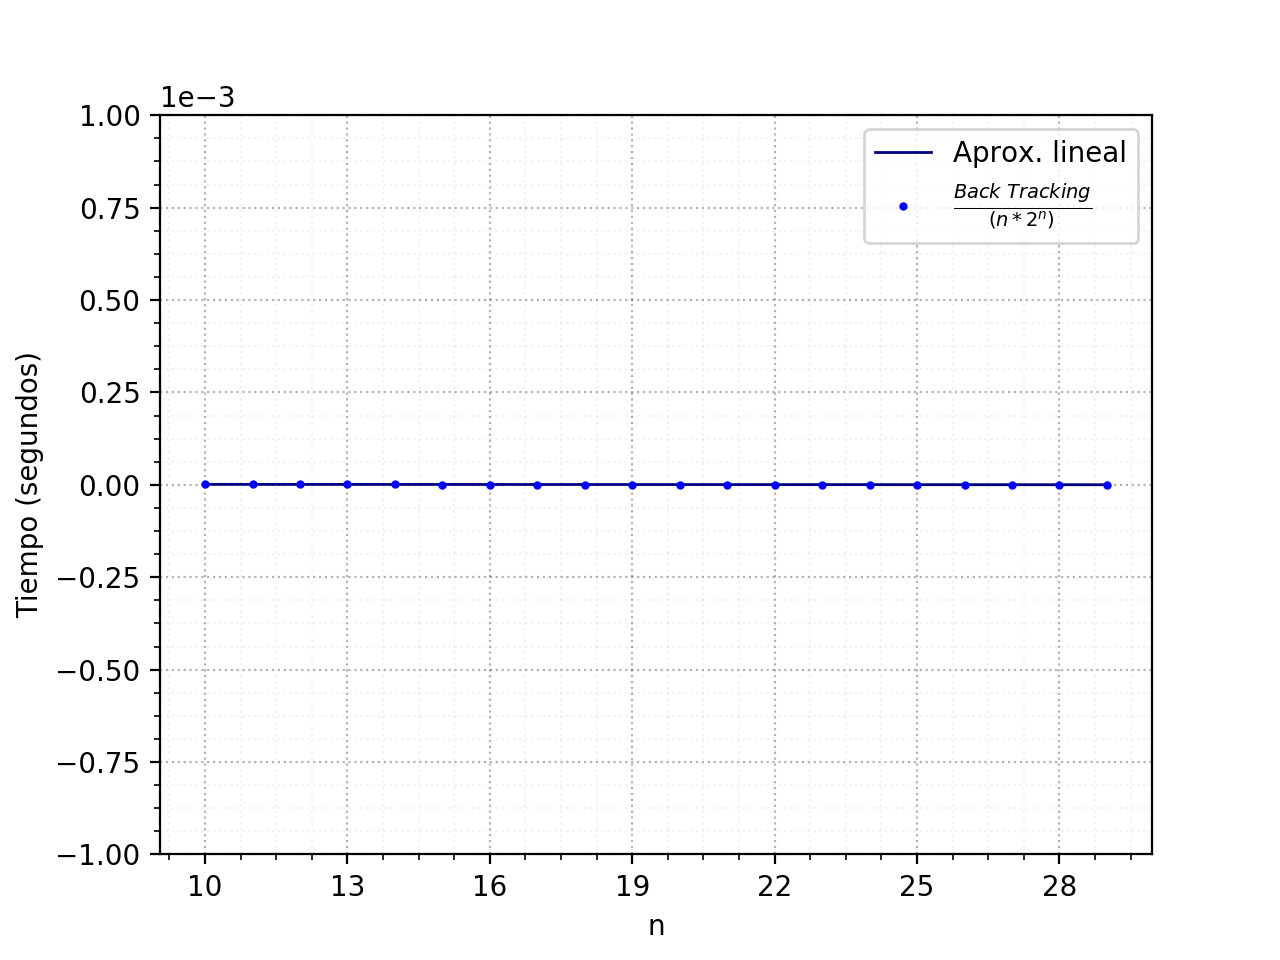
\includegraphics[width=0.5\textwidth]{bt-div-cota}
	\caption{\footnotesize Segundos consumidos en función de la cantidad de elementos de $values$ dividido $n*2^n$}
	\label{fig:plot-bt-div-cota}
\end{figure}

\subsection{Programación Dinámica}
\begin{figure}[H]
	\centering
	\begin{minipage}{0.48\textwidth}
		\centering
		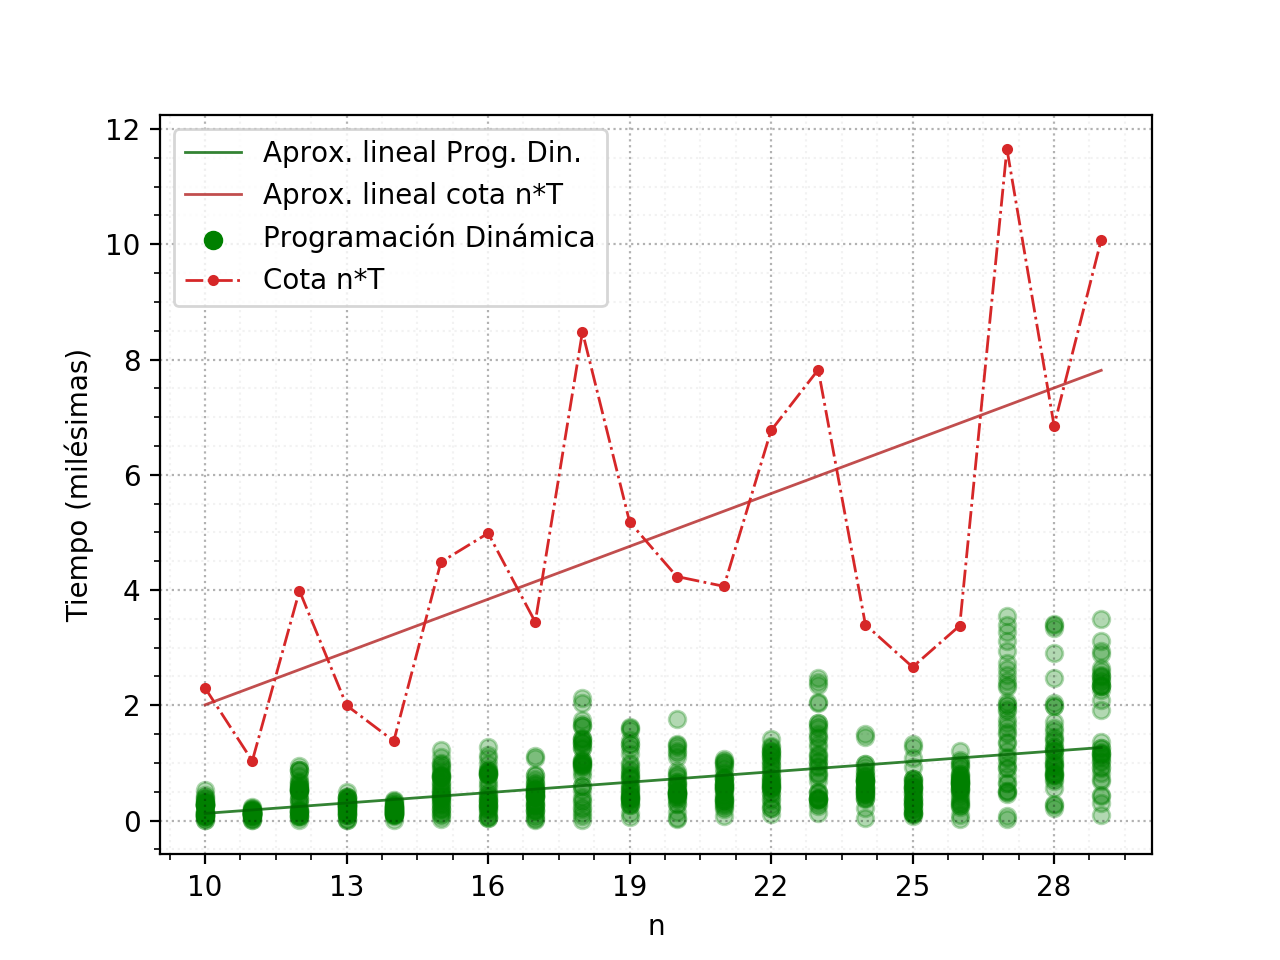
\includegraphics[width=1\textwidth]{pd-and-cota}
		\caption{\footnotesize Segundos consumidos (en escala lineal) en función de la cantidad de elementos de $values$.}
		\label{fig:plot-bf-and-cota}
	\end{minipage}%
	\hspace{0.03\textwidth}
	\begin{minipage}{0.48\textwidth}
		\centering
		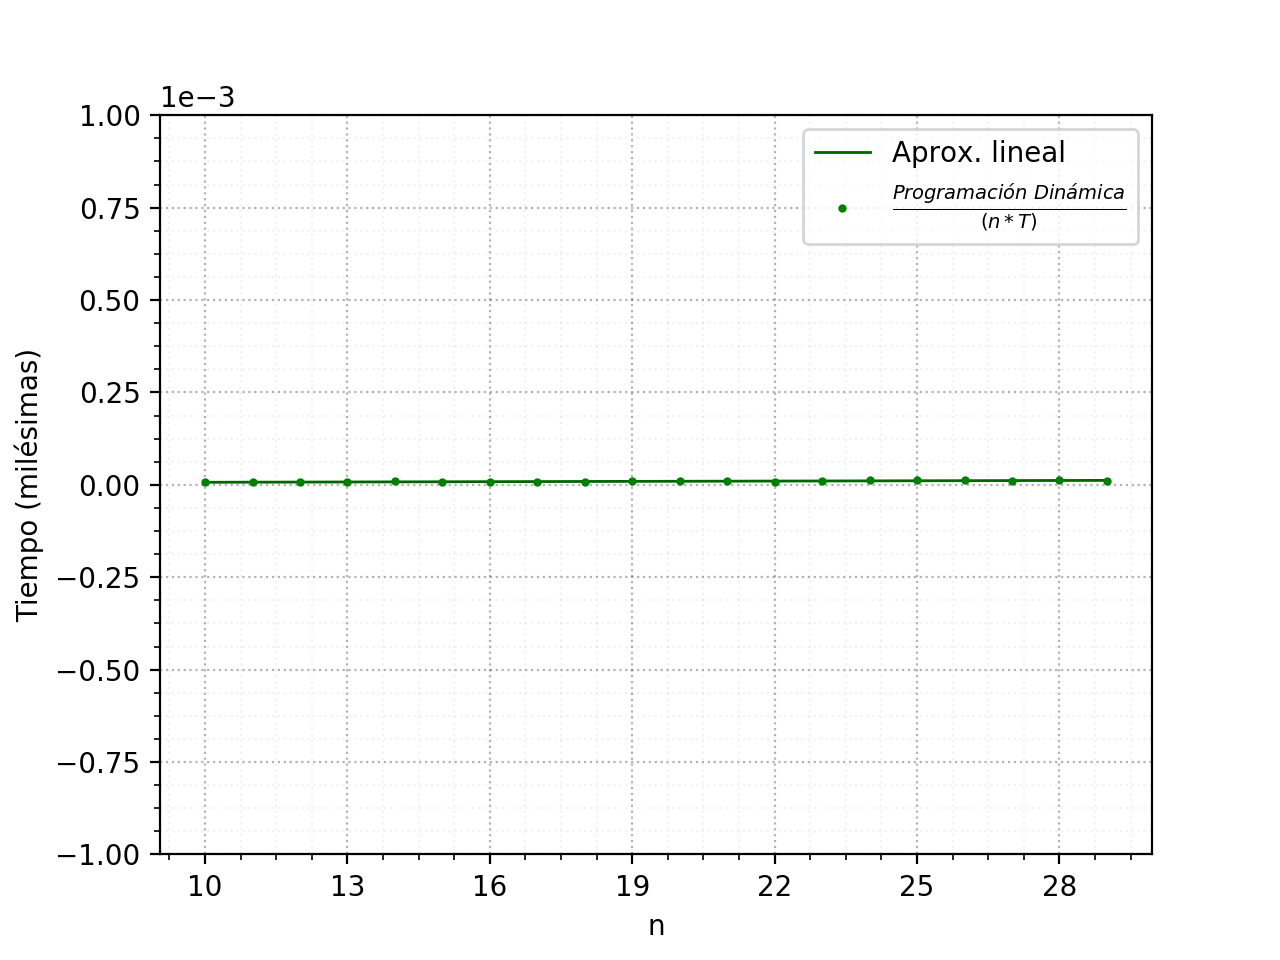
\includegraphics[width=1\textwidth]{pd-div-cota}
		\caption{\footnotesize Segundos consumidos en función de la cantidad de elementos de $values$ dividido $n*T$}
		\label{fig:plot-bf-and-cota-log}
	\end{minipage}%
\end{figure}